
After starting metaOmics, 
the first page is the metaOmics setting page as shown in Figure~\ref{fig:GUIsetting}.  
There are 4 tabs on top of the page (at position {\color{red} (1)}): Setting, Preprocessing, Saved Data and Toolsets.
Below the 4 tabs, 
the first header is the session information.
{
\color{blue}
Why do we need session information?
}
The second header is Directory for Saving Output Files (at position {\color{red} (2)}).
By clicking ``$\ldots$",
user can set default working directory, in which all the meta-analysis results will be saved.
Users can view their current working directory on the top right corner (at position {\color{red} (3)}).
The third header is Toolsets (at position {\color{red} (4)}),
here users can view if individual packages are installed.
If the packages are installed, there is a checked installed status.
Otherwise, users can install individual package by clicking install blue button.
Position {\color{red} (5)} shows the current active dataset, which will be introduced in Section~\ref{sec:procedure}~\ref{sec:active}. 
 
\begin{figure}[H]
\begin{center}
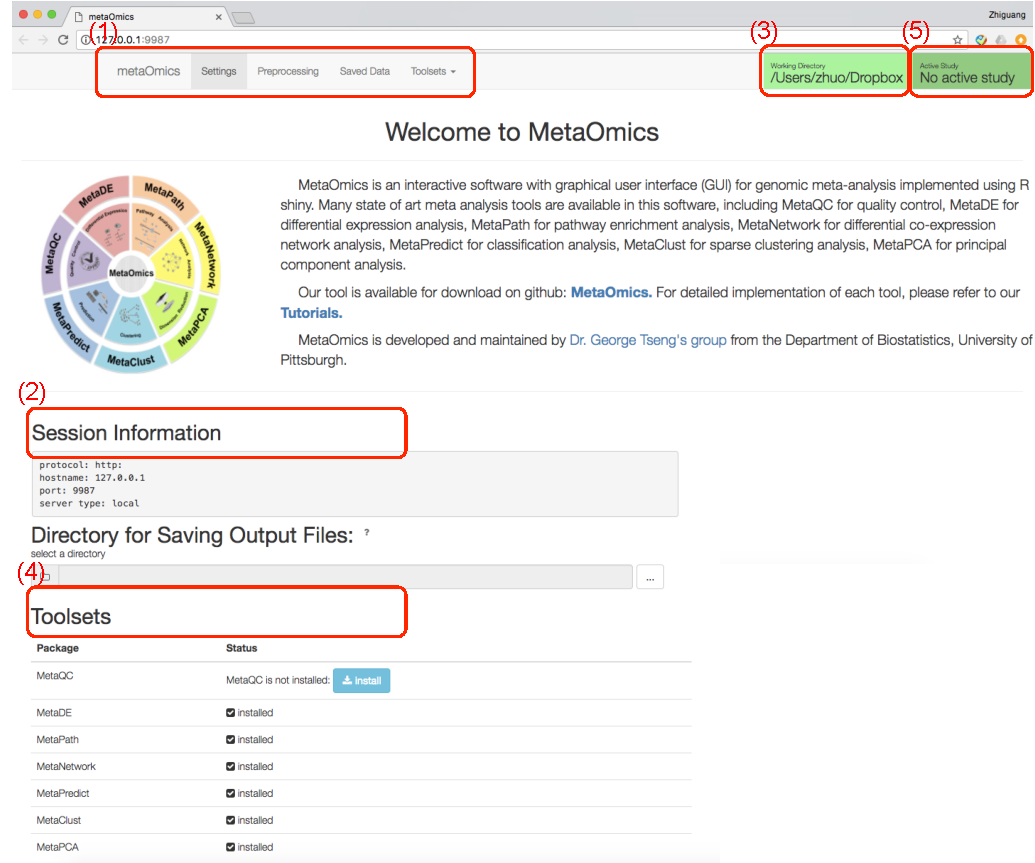
\includegraphics[scale=0.4]{./figure/preprocessing/GUIsetting}
\caption{GUI setting page}
\label{fig:GUIsetting}
\end{center}
\end{figure}

\subsection{Preprocessing}

In this subsection, we will introduce how to upload your dataset into the MetaOmics suit such that the functional modules can be utilized.
The R package for preprocessing module can be found \url{https://github.com/metaOmic/preproc}.

\subsubsection{Procedure}
\label{sec:procedure}

\begin{steps}
\item \textbf{Uploading data:}

\begin{figure}[!htbp]
\begin{center}
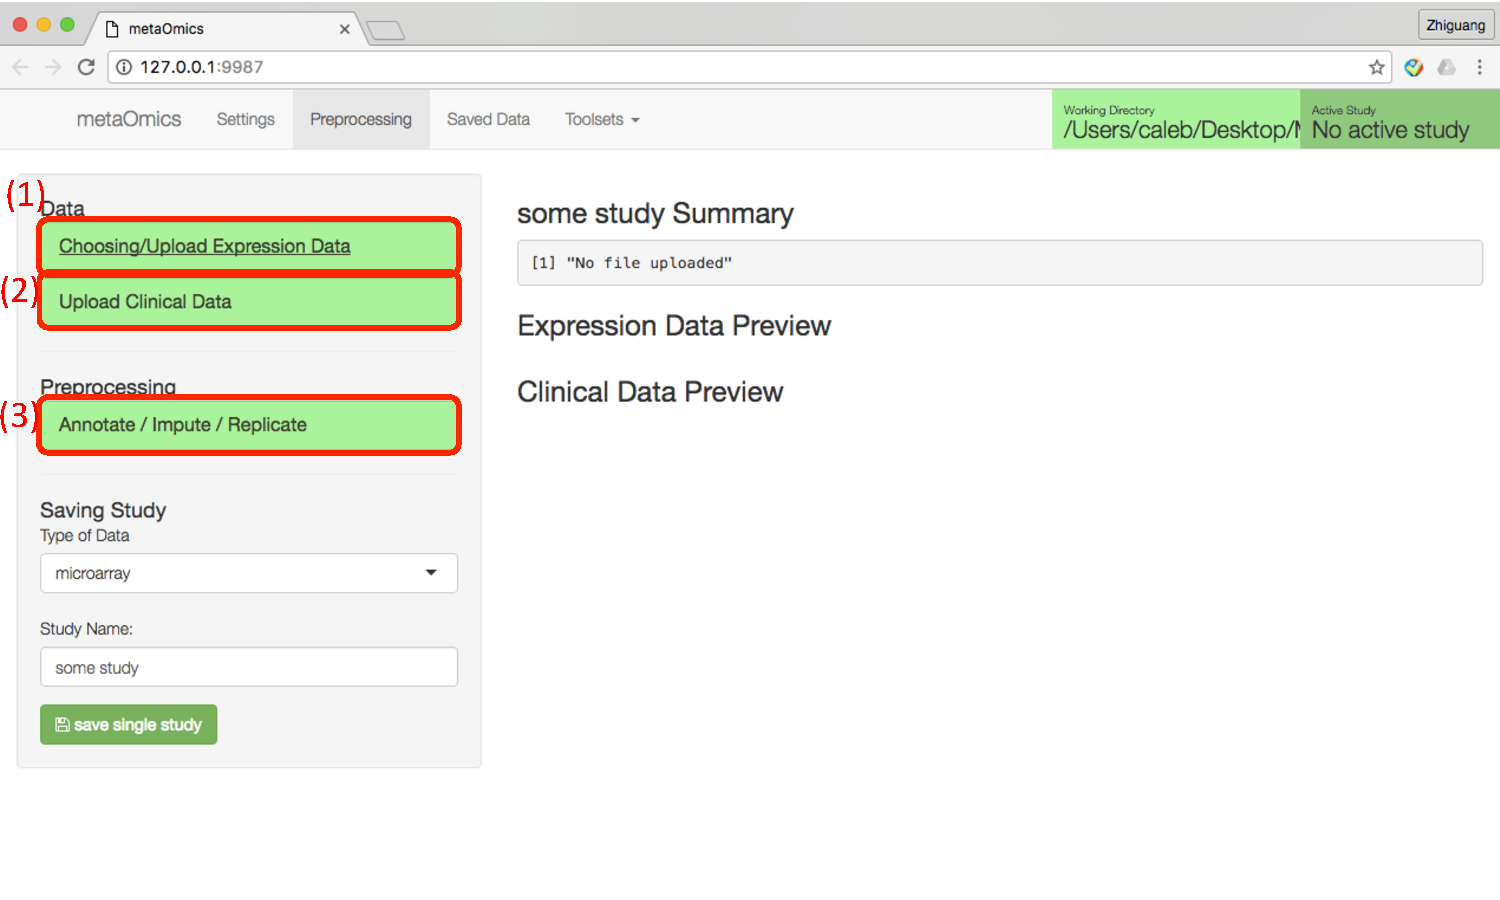
\includegraphics[scale=0.4]{./figure/preprocessing/GUIpreprocessing}
\caption{GUI Preprocessing page}
\label{fig:GUIpreprocessing}
\end{center}
\end{figure}

After clicking the Preprocessing tab as in Figure~\ref{fig:GUIpreprocessing},
users are able to upload their datasets via the tab ``Choosing/Upload Expression Data" as in Figure~\ref{fig:GUIpreview} (at position {\color{red} (1)}).
The data should be prepared according to Section~\ref{sec:dataPrepare}.
Users may optionally upload Clinical Data (at position {\color{red} (2)}), depending on biological purpose.
All MetaOmics modules except for MetaClust  require external clinical labels.
An example data can be found within MetaOmics folder ``metaOmcis/data/example/leukedia".
The MetaOmics suit also provides handlers (at position {\color{red} (3)}) for feature annotation, missing value imputation and multiple probe same genes.
After uploading is complete,
users can preview their data on the right hand side of the page as Figure~\ref{fig:GUIpreview}.

\item \textbf{Preprocessing:}


There are several expression data parsing options available on the left panel of Figure~\ref{fig:GUIpreview}.
A complete introduction of these options is available at the end of this subsection.
The right hand side of Figure~\ref{fig:GUIpreview} shows the summary statistics of uploaded data and preview of the data matrix.
There is a search box such that the user can search their favorite genes.

\begin{figure}[H]
\begin{center}
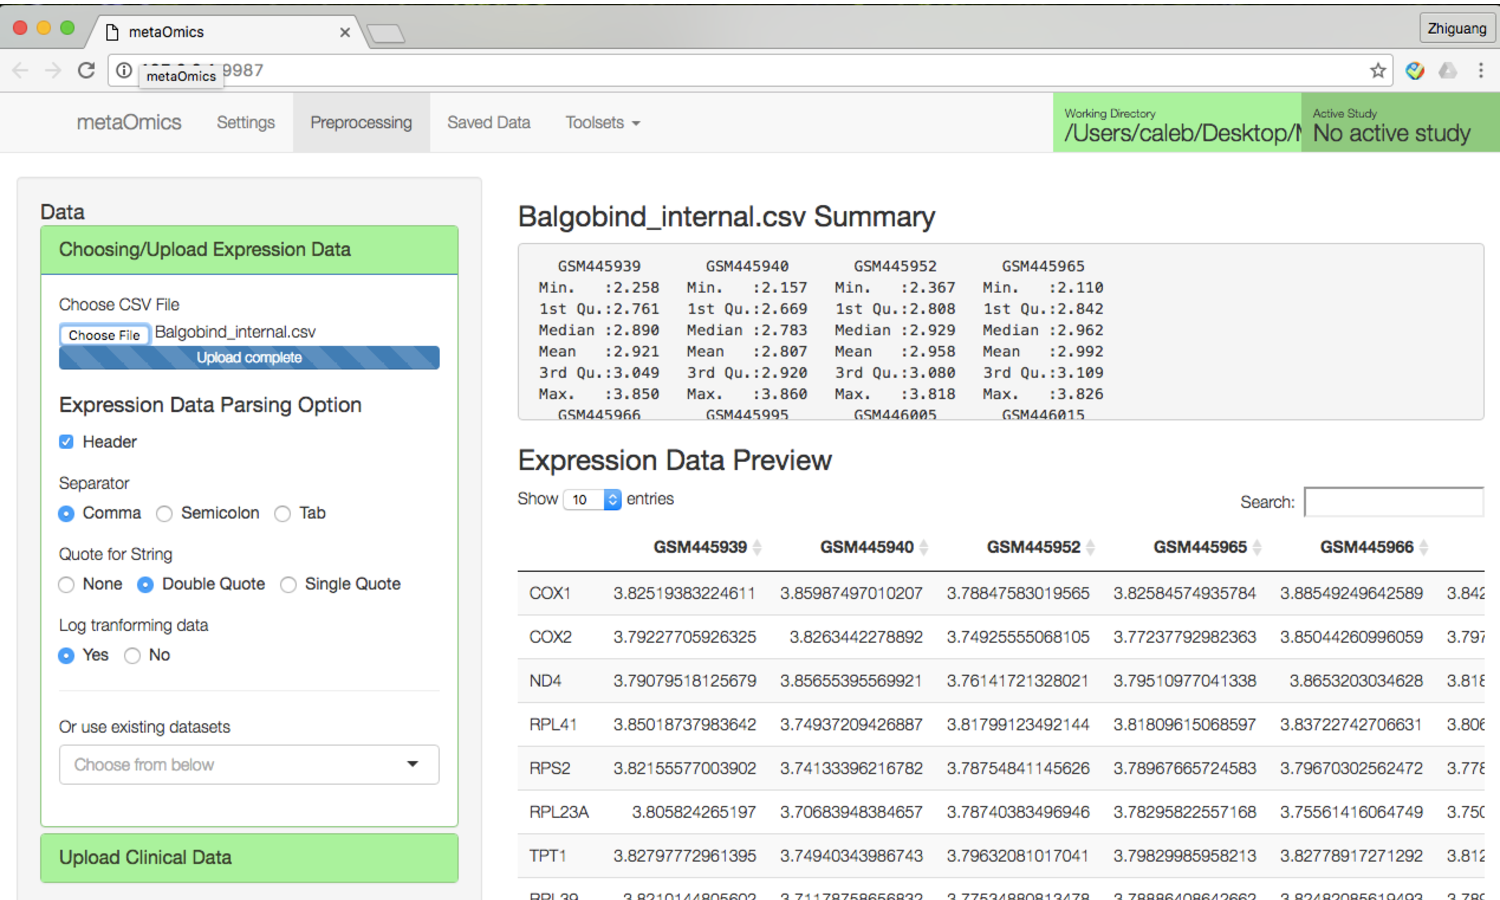
\includegraphics[scale=0.4]{./figure/preprocessing/GUIpreview}
\caption{Uploading individual studies}
\label{fig:GUIpreview}
\end{center}
\end{figure}
After users upload clinical data (e.g. case control labels) and specify type of data and study name.
They can click ``save single study" button, single study will be saved.

\item \textbf{Saved Data:}

After uploading multiple studies w/o clinical data,
users can turn to the Saved Data tab.
Users should select multiple datasets as Figure~\ref{fig:GUImerge} (at position {\color{red} (2)}).
After specifying filtering criteria, enter merged study name and click on the ``Merge from Selected Datasets" (at position {\color{red} (1)}).
A merged dataset will appear on the  ``List of saved data" panel (at position {\color{red} (2)}).

\begin{figure}[H]
\begin{center}
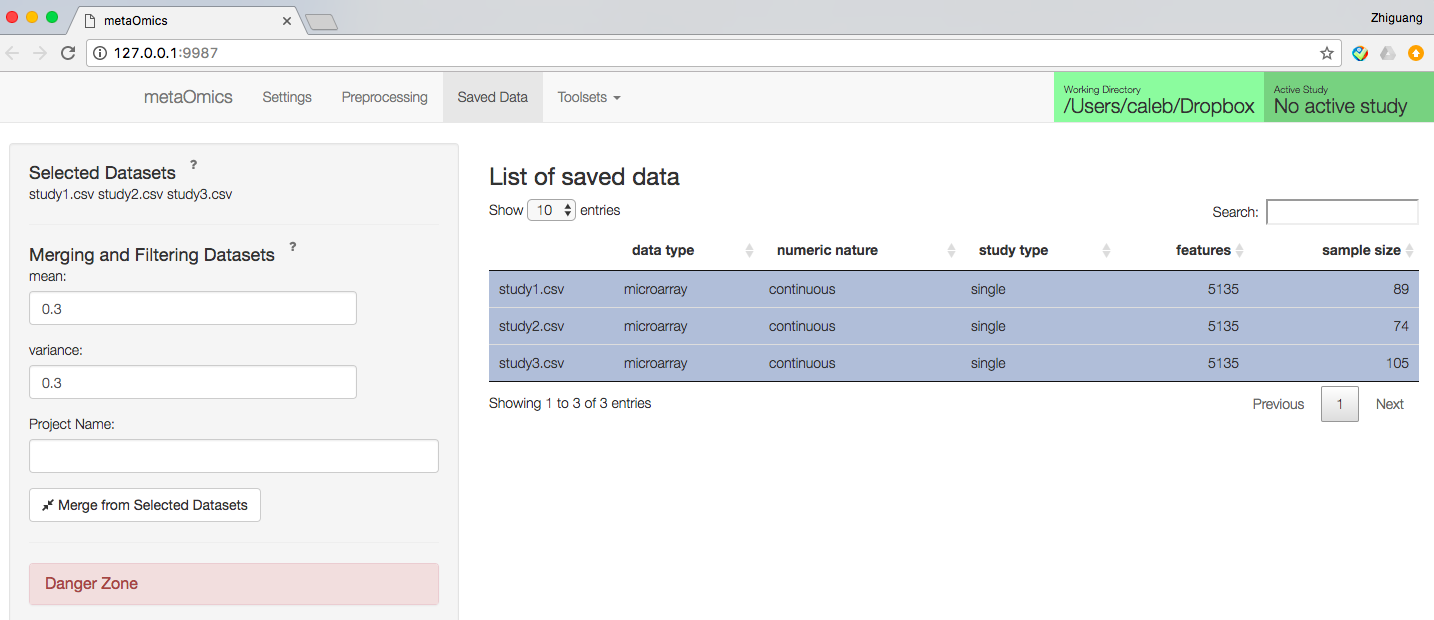
\includegraphics[scale=0.4]{./figure/preprocessing/GUImerge}
\caption{Merge from selected datasets}
\label{fig:GUImerge}
\end{center}
\end{figure}

\item \textbf{Make merged Dataset Active:}

\label{sec:active}
The last thing to do before using meta-analytic toolsets is to select merged data and click on 
``Make your dataset Active Dataset" - A big green button in Figure~\ref{fig:active}.
Then the merged data becomes active study and shows up on the top right corner.
The active dataset serves as the input for all other MetaOmics modules.
If users want to delete a dataset, just click ``Delete Selected Data" button after selecting the dataset.

\begin{figure}[H]
\begin{center}
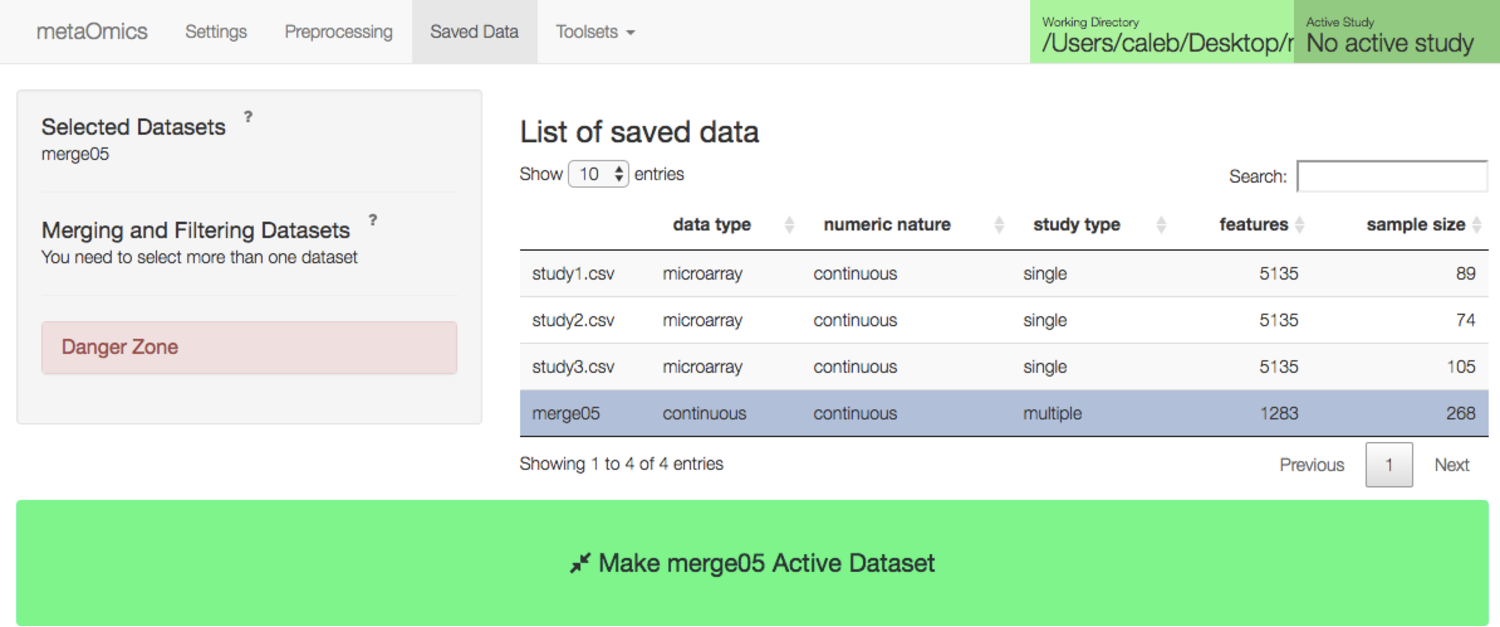
\includegraphics[scale=0.4]{./figure/preprocessing/GUImarkActive}
\caption{Make merged Dataset Active}
\label{fig:active}
\end{center}
\end{figure}



\end{steps}

\textbf{Complete List of Options:} 
\begin{enumerate}
\item Upload expression data:
\begin{itemize}
\item Header: should be checked if the input file includes a header.
\item Separator: indicates what type of separator is used for the data matrix.
\item Quote for String: how is the data matrix quoted.
\item Log transforming data: if you want to perform log transformation of your data, check yes.
\item Use existing datasets: if you want to load a dataset previously uploaded, you can choose from the checklist.
\end{itemize}
\item Annotation/impute/Replicate:
\begin{itemize}
\item Annotation: possible ID type can be Gene Symbol (default), Probe ID, reference sequence ID, entrez ID.
\item Impute: if selected, missing value imputation will be performed by k-nearest neighbor algorithm.
\item Replicate Handling: if selected, if the same gene symbol maps to multiple probes, the probe with the largest inner quantile range (IQR) will be selected
as a representative for this gene.
\end{itemize}
\item Saved Data, Merging and Filtering Datasets:
\begin{itemize}
\item Mean: the criteria such that how many percent of genes will be filtered out based on sum of mean ranks (e.g. 0.3 represent 30\%).
\item Variance: after the Mean filtering, the criteria such that how many percent of genes will be filtered out based on sum of variance ranks (e.g. 0.3 represent 30\%).
\item Study Name: dataset name after merging. This name will appear in the list of saved data table.
\item Merge from Selected Datasets: perform filtering and merging.
\end{itemize}
\item Danger zone:
\begin{itemize}
\item Delete Selected Data: the selected data will be delete permanently if clicked, so please be cautious.
\end{itemize}

\end{enumerate}



